\documentclass[8pt, letterpaper]{article}
\usepackage[ngerman]{babel}
\usepackage{graphicx}
\usepackage[utf8]{inputenc}
\usepackage{gensymb}
\usepackage{blindtext}
\usepackage{geometry}
\usepackage{fancyhdr}
\usepackage{url}
\usepackage{seqsplit}
\usepackage{hyperref}

\usepackage{courier} %% Sets font for listing as Courier.
\usepackage{listings, xcolor}
\lstset{
tabsize = 4, %% set tab space width
showstringspaces = false, %% prevent space marking in strings, string is defined as the text that is generally printed directly to the console
numbers = left, %% display line numbers on the left
commentstyle = \color{green}, %% set comment color
keywordstyle = \color{blue}, %% set keyword color
stringstyle = \color{red}, %% set string color
rulecolor = \color{black}, %% set frame color to avoid being affected by text color
basicstyle = \small \ttfamily , %% set listing font and size
breaklines = true, %% enable line breaking
numberstyle = \tiny,
}

\graphicspath{{images/}}
\setlength{\parindent}{0cm}
\bibliographystyle{gerplain}
\geometry{letterpaper, margin=1in}
\pagestyle{fancy}

\lhead{Jakob Kirsch}
\rhead{
\includegraphics[width=3cm]{logo}}

% \title{}
% \author{Jakob Kirsch}
% \date{\parbox{\linewidth}{\centering%
%   \today\endgraf\bigskip
%   Fach: \endgraf\medskip
%   Betreuer: \endgraf\medskip
%}}

\begin{document}

% \maketitle
% \newpage
% \tableofcontents
% \newpage

Wenn man dem letzten Blatt gefolgt ist, hat man sehr wahrscheinlich die folgende Meldung gesehen:

\begin{center}
  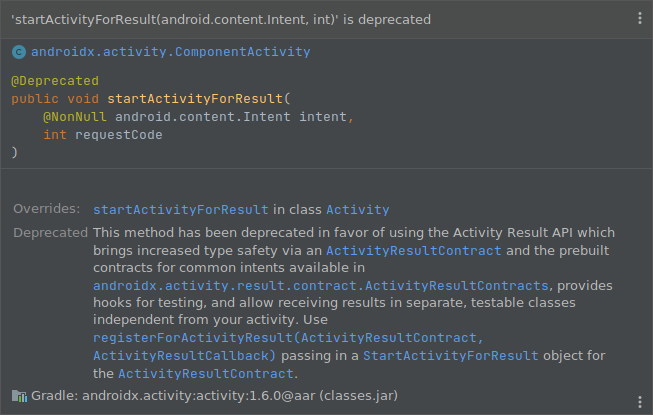
\includegraphics{deprecated}
\end{center}

Anscheinent soll man jetzt \texttt{ActivityResultContract}s nutzen.

Also deklarieren wir innerhalb der Klasse (wo wir auch \texttt{Button}s etc. deklarieren) einen \texttt{ActivityResultLauncher} namens \texttt{launcher}. Das \texttt{<Intent>} besagt, dass wir unsere Daten als \texttt{Intent}s übergeben.

\begin{center}
  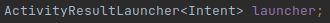
\includegraphics{declare}
\end{center}

Innerhalb der \texttt{onCreate} Methode instantiieren wir dann diesen Launcher. Dafür registrieren wir mit \texttt{registerForActivityResult} einen Handler, der das Ergebniss der anderen Activity verarbeitet, indem wir ihm ein \texttt{ActivityResultCallback<ActivityResult>} geben, welches ein \texttt{ActivityResult} entgegennimmt, das sowohl den Statuscode (hat es funktioniert?) als auch die Daten enthält.

\begin{center}
  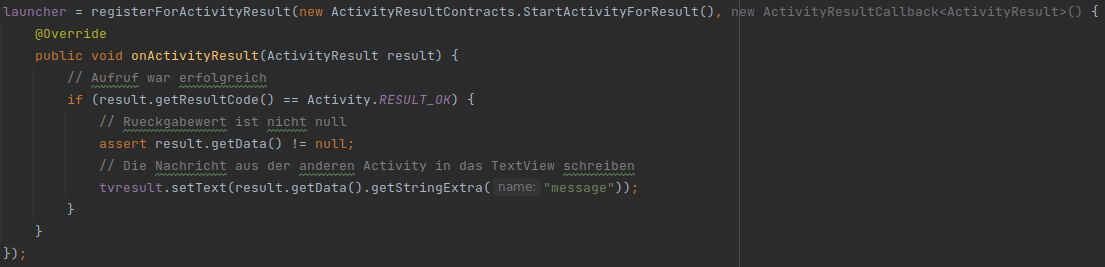
\includegraphics[width=18cm]{instanciate}
\end{center}

Um dann die zweite Activity zu starten nutzen wir nicht mehr \texttt{startActivityForResult(intent, code)} sonder \texttt{launcher.launch(intent)}.
Das wars auch schon. Hier ist nochmal der gesammte Code eines Beispiels:
\pagebreak

MainActivity.java
\begin{lstlisting}[language = Java , frame = trBL , firstnumber = last , escapeinside={(*@}{@*)}]
package de.jakob.myapplication;

import androidx.activity.result.ActivityResult;
import androidx.activity.result.ActivityResultCallback;
import androidx.activity.result.ActivityResultLauncher;
import androidx.activity.result.contract.ActivityResultContracts;
import androidx.appcompat.app.AppCompatActivity;

import android.app.Activity;
import android.content.Intent;
import android.os.Bundle;
import android.view.View;
import android.widget.Button;
import android.widget.TextView;

public class MainActivity extends AppCompatActivity {
    Button bnext;
    TextView tvresult;
    ActivityResultLauncher<Intent> launcher;

    @Override
    protected void onCreate(Bundle savedInstanceState) {
        super.onCreate(savedInstanceState);
        setContentView(R.layout.activity_main);

        launcher = registerForActivityResult(new ActivityResultContracts.StartActivityForResult(), new ActivityResultCallback<ActivityResult>() {
            @Override
            public void onActivityResult(ActivityResult result) {
                // Aufruf war erfolgreich
                if (result.getResultCode() == Activity.RESULT_OK) {
                    // Rueckgabewert ist nicht null
                    assert result.getData() != null;
                    // Die Nachricht aus der anderen Activity in das TextView schreiben
                    tvresult.setText(result.getData().getStringExtra("message"));
                }
            }
        });

        bnext = findViewById(R.id.back_button);
        tvresult = findViewById(R.id.textView);
        bnext.setOnClickListener(new View.OnClickListener() {
            @Override
            public void onClick(View view) {
                Intent intent = new Intent(MainActivity.this, SecondActivity.class);
                launcher.launch(intent);
            }
        });
    }
}
\end{lstlisting}

% \newpage
% \bibliography{refs}

\end{document}
